\documentclass[11pt]{article}

\usepackage[a4paper,margin=1in]{geometry}
\usepackage{microtype}
\usepackage{graphicx}
\usepackage{booktabs}
\usepackage{longtable}
\usepackage{array}
\usepackage{amsmath}
\usepackage{siunitx}
\usepackage[authoryear,round]{natbib}
\usepackage[colorlinks=true,linkcolor=blue,citecolor=blue,urlcolor=blue]{hyperref}
\usepackage[font=small,labelfont=bf]{caption}
\usepackage{subcaption}
\usepackage{tikz}
\usetikzlibrary{arrows.meta,positioning}

\sisetup{detect-all}
\graphicspath{{../}}
\setlength{\emergencystretch}{3em}

\title{\textbf{Chandra X-ray Luminosity and Halo-Mass Scaling Relations}\\
\large A weak-lensing calibrated analysis of CLASH and LoCuSS clusters}
\author{Advanced Observational Astrophysics Final Project}
\date{May 2026}

\newcommand{\Mfive}{\ensuremath{M_{500}}}
\newcommand{\Rfive}{\ensuremath{R_{500}}}
\newcommand{\Lx}{\ensuremath{L_{\mathrm{X}}}}
\newcommand{\Tx}{\ensuremath{T_{\mathrm{X}}}}
\newcommand{\Ez}{\ensuremath{E(z)}}

\begin{document}
\maketitle

\begin{abstract}
This project measures X-ray luminosity--mass, temperature--mass, and luminosity--temperature scaling relations for a Chandra sample with weak-lensing mass calibration. The working sample begins with CLASH and LoCuSS clusters, removes seven visually unsuitable systems, processes 23 clusters through a Chandra/CIAO imaging and spectral pipeline, and adopts an 18-cluster main scaling sample after spectral quality control. Temperatures and luminosities are measured from per-ObsID Sherpa spectral fits using an absorbed APEC intracluster-medium model, blank-sky particle backgrounds renormalized at 9.5--12 keV, and explicit sky-background components. Scaling relations are fit with \texttt{linmix} at fixed self-similar redshift evolution. For the full-\Rfive{} baseline sample, the fitted slopes are $\beta_{\Lx-M}=1.08^{+0.45}_{-0.48}$ and $\beta_{\Tx-M}=0.50^{+0.29}_{-0.27}$, with intrinsic scatters of 0.169 dex and 0.117 dex. A core-excised $0.15$--$1.0\Rfive$ branch gives consistent mass-based slopes within the present uncertainties. The main conclusion is that this repository now implements a complete, reproducible chain from Chandra data products to weak-lensing calibrated scaling-relation inference, while the final precision remains limited by sample size, background systematics, and a few high-temperature or low-quality spectra.
\end{abstract}

\section{Scientific Motivation}

Galaxy clusters are extreme laboratories for both cosmology and baryonic astrophysics. On the cosmological side, they are the most massive gravitationally bound systems in the late-time Universe, so their abundance and growth trace the formation of large-scale structure. On the baryonic side, the same dark-matter halos contain hot gas, galaxies, metals, magnetic fields, shocks, turbulence, and feedback from active galactic nuclei. A cluster therefore lets us ask two linked questions in one object: how massive is the halo, and how do baryons behave inside that halo?

For an oral presentation, the core physical chain is simple: halo mass sets the depth of the gravitational potential; the potential heats the intracluster gas; the hot gas emits X-rays; and the measured X-ray luminosity and temperature can then be calibrated against halo mass. The project goal is to measure that chain quantitatively by fitting \Lx--\Mfive{}, \Tx--\Mfive{}, and \Lx--\Tx{} relations.

\subsection{Definitions and Physical Chain}

\Mfive{} is the mass enclosed within \Rfive{}, the radius where the mean enclosed density is 500 times the critical density at the cluster redshift. The factor \Ez{} describes the redshift evolution of the Hubble expansion rate and therefore the characteristic density scale of collapsed halos. The intracluster medium, or ICM, is the diffuse plasma trapped by the cluster potential; its typical temperature is $10^7$--$10^8$ K, which places much of its thermal emission in the X-ray band.

Temperature is the more direct gravitational observable. If the halo is more massive, the potential well is deeper, and virial equilibrium requires a hotter gas. Luminosity is also mass-related, but it depends strongly on gas density because thermal bremsstrahlung scales approximately as $n_e^2\Lambda(T)$, where $n_e$ is the electron density and $\Lambda(T)$ is the cooling function. This density-squared dependence is why \Lx{} is especially sensitive to cool cores, gas clumping, feedback, and mergers.

\begin{figure}[t]
  \centering
  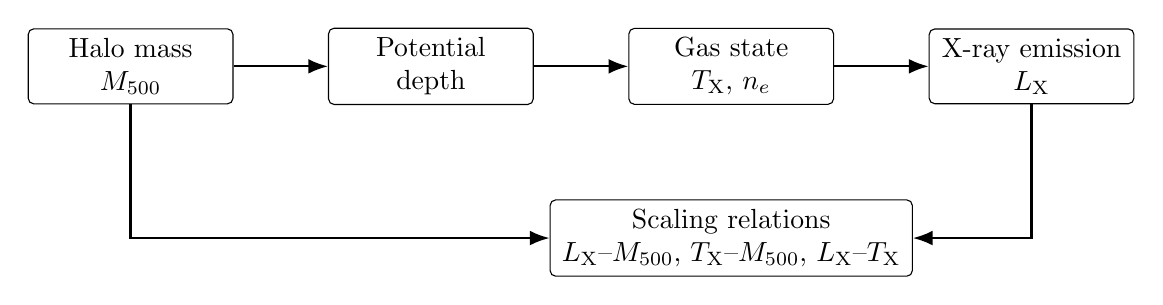
\begin{tikzpicture}[
    node distance=1.2cm,
    box/.style={draw, rounded corners=2pt, align=center, minimum width=2.6cm, minimum height=0.9cm},
    arrow/.style={-{Latex[length=2.5mm]}, thick}
  ]
    \node[box] (m) {Halo mass\\\Mfive};
    \node[box, right=of m] (phi) {Potential\\depth};
    \node[box, right=of phi] (gas) {Gas state\\\Tx{}, $n_e$};
    \node[box, right=of gas] (lx) {X-ray emission\\\Lx};
    \node[box, below=of gas, minimum width=4.6cm] (fit) {Scaling relations\\\Lx--\Mfive{}, \Tx--\Mfive{}, \Lx--\Tx};
    \draw[arrow] (m) -- (phi);
    \draw[arrow] (phi) -- (gas);
    \draw[arrow] (gas) -- (lx);
    \draw[arrow] (lx.south) |- (fit.east);
    \draw[arrow] (m.south) |- (fit.west);
  \end{tikzpicture}
  \caption{Conceptual chain used in the talk: mass sets the potential, the potential sets the thermodynamic state of the gas, and the gas produces the X-ray observables used in the scaling-relation fit.}
  \label{fig:physical-chain}
\end{figure}

\subsection{Self-Similar Expectation and Real Scatter}

In the simplest self-similar picture, clusters differ only by mass and redshift-dependent density scale \citep{kaiser1986,arnaud2005}. Virial equilibrium predicts
\begin{equation}
  T_{\mathrm{X}} \propto M_{500}^{2/3} E(z)^{2/3},
\end{equation}
and bolometric bremsstrahlung luminosity gives approximately
\begin{equation}
  L_{\mathrm{X}} \propto M_{500}^{4/3} E(z)^2.
\end{equation}
Equivalently, the self-similar bolometric luminosity--temperature slope is $L_{\mathrm{X}}\propto E(z)T_{\mathrm{X}}^2$. This is the clean theoretical baseline to keep in mind during the presentation.

Real clusters deviate from these ideal scalings because gas cooling, AGN feedback, merger shocks, core entropy structure, gas-fraction variation, gas clumping, projection, and asphericity change the thermodynamic state of the ICM \citep{pratt2009,mantz2010,maughan2012}. Observationally, a scaling relation is therefore not just a line; it is a mean trend plus intrinsic scatter. That scatter is not merely a nuisance term. It contains information about dynamical state, baryonic physics, and measurement systematics. These effects motivate explicit quality control and a comparison between full-aperture and core-excised measurements.

\subsection{From Background to This Project}

The mass scale used here is deliberately independent of the X-ray observables. CLASH cluster masses are taken from the weak-lensing analysis of \citet{umetsu2016}, while LoCuSS masses are taken from \citet{okabe2016}. Using weak-lensing \Mfive{} avoids calibrating X-ray observables against X-ray hydrostatic masses, which would partially share the same physical assumptions and systematics.

The project then connects the background physics to a reproducible measurement chain. First, select clusters with lensing-based halo masses. Second, reduce their Chandra observations with CIAO and preserve per-ObsID spectral responses. Third, model source and background spectra to measure \Tx{} and model-derived \Lx{}. Finally, fit the scaling relations with \texttt{linmix}, including measurement errors and intrinsic scatter. The final scientific question is: how well do the observable properties of hot gas trace the underlying halo mass once real cluster physics and data quality are accounted for?

\section{Sample and Data Products}

The parent working sample combines CLASH and LoCuSS clusters with Chandra coverage and weak-lensing mass measurements. Seven morphologically unsuitable or visually/aspherically problematic objects are removed before the main Chandra processing: Abell 0115, Abell 0141, Abell 0521, Abell 2813, MACSJ0416.1--2403, MACSJ0717.5+3745, and MACSJ1149.5+2223. The remaining 23 clusters pass through the imaging and spectral pipeline. After the spectral quality pass, five systems are excluded from the main scaling sample: Abell 0697, Abell 0750, MS2137--2353, RXJ1347.5--1145, and ZwCl 0857.9+2107. These objects are retained in the archive but not used in the baseline regression because of failed all-ObsID fits, extreme or unstable temperatures, poor reduced statistics, or inconsistent external reference comparisons.

The adopted main sample therefore contains 18 clusters: 11 labeled good, 4 acceptable, and 3 high/suspect but retained. The high retained systems, including Abell 0611, MACSJ0647.7+7015, and MACSJ1206.2--0847, are carried through the baseline analysis and tested through stricter quality subsets and leave-one-out refits rather than being silently removed.

The canonical full-aperture table is \texttt{output/products/spectral/spectral\_summary.csv}. A merged final report table, \texttt{output/products/final\_spectral\_table.csv}, records the 18 retained clusters with redshift, weak-lensing mass, \Rfive{}, full-\Rfive{} spectral quantities, core-excised spectral quantities, and quality labels.

\section{Chandra Reduction and Spectral Measurement}

The repository implements a staged Chandra workflow. Each ObsID is reprocessed with CIAO \texttt{chandra\_repro}; merged images are then constructed with \texttt{merge\_obs} for visualization, X-ray peak finding, and point-source detection. Compact sources are identified with \texttt{wavdetect} and masked. The merged imaging products are used for QA and region definition, but spectral fitting is done from per-ObsID extractions so that each spectrum keeps the correct ARF and RMF response.

Spectra are extracted with CIAO \texttt{specextract} and fit jointly in Sherpa \citep{fruscione2006}. The source model is an absorbed APEC plasma, with Galactic $N_{\mathrm{H}}$ and redshift fixed from the cluster table and abundance fixed to $0.3\,Z_\odot$ in the main run. The fit band is 0.7--7.0 keV. The statistical model is WSTAT, appropriate for Poisson source spectra with measured background. Minimal grouping is used for WSTAT fits.

The background model is a central technical part of the project. Particle background is handled with CIAO blank-sky spectra, reprojected to the observation and renormalized through the 9.5--12 keV count-rate ratio, where cluster thermal emission is weak and the particle background dominates. The sky background is represented by source-region components for the local hot bubble, Galactic halo, and cosmic X-ray background. The default branch uses a fixed-shape XRB treatment, with flexible tests for clusters where the full-\Rfive{} behavior warrants them. This strategy follows the broad logic of Chandra cluster background work in the literature \citep[e.g.][]{vikhlinin2009,donahue2014}, while keeping the implementation reproducible in the project scripts.

Two apertures are measured. The baseline branch uses the full \Rfive{} source region. The comparison branch uses $0.15$--$1.0\Rfive$, removing the central core in a literature-style way. Full-\Rfive{} and core-excised products are kept in separate output directories so that aperture definitions cannot be mixed silently. Core-excised luminosity intervals use Sherpa \texttt{sample\_energy\_flux}. Core-excised temperature confidence intervals are not stored in the current JSON products, so \Tx{}-based core-excised scaling fits use a documented 10 percent temperature-error fallback.

\begin{figure}[t]
  \centering
  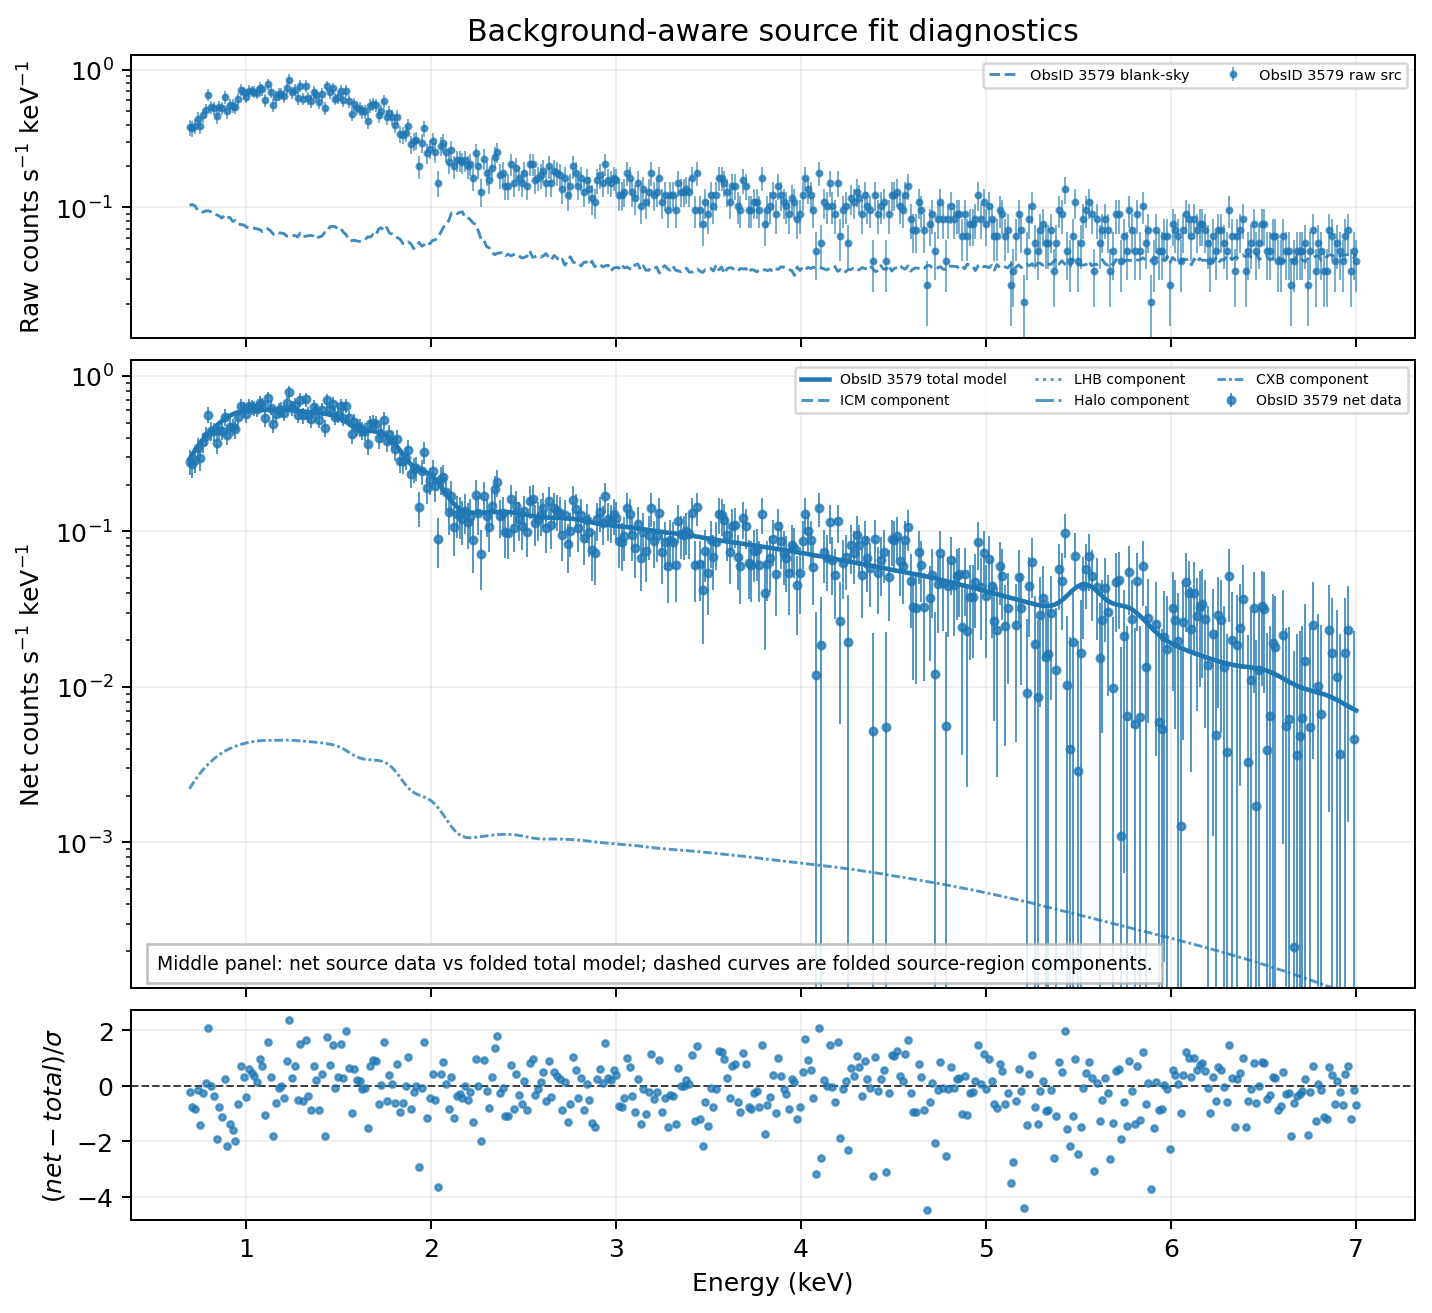
\includegraphics[width=0.95\linewidth]{output/figures/spectral/Abell_0209_fit.png}
  \caption{Representative full-\Rfive{} spectral QA product for Abell 0209. The updated plot separates raw source and background behavior from the net source spectrum and folded source-region model, avoiding the visual offset that affected earlier WSTAT diagnostic plots.}
  \label{fig:spectral-qa}
\end{figure}

\section{Scaling-Relation Model}

Scaling relations are fit using \texttt{linmix}, the Bayesian linear-regression method of \citet{kelly2007}. The fits use base-10 logarithms, account for measurement errors in both axes, and report intrinsic scatter in dex in the dependent variable at fixed independent variable. The regression model is
\begin{equation}
  \log_{10}\left[\frac{Y}{E(z)^{\gamma}}\right]
  = \alpha + \beta \log_{10}\left(\frac{X}{X_{\mathrm{piv}}}\right).
\end{equation}
The fixed-evolution relations are
\begin{align}
  E(z)^{-2} L_{\mathrm{X,bol}} &= A \left(\frac{M_{500}}{3\times10^{14}M_\odot}\right)^\beta,\\
  E(z)^{-2/3} T_{\mathrm{X}} &= A \left(\frac{M_{500}}{3\times10^{14}M_\odot}\right)^\beta,\\
  E(z)^{-1} L_{\mathrm{X,bol}} &= A \left(\frac{T_{\mathrm{X}}}{5\,\mathrm{keV}}\right)^\beta.
\end{align}
The fixed exponents match the self-similar comparison convention. \Mfive{} errors are taken from the literature mass references encoded in the canonical products. \Rfive{} uncertainties are propagated from \Mfive{} as aperture provenance and are not added as independent regression errors.

\section{Results}

\subsection{Full-\texorpdfstring{$R_{500}$}{R500} Baseline}

The main full-\Rfive{} scaling sample contains 18 clusters. Figure~\ref{fig:full-scaling} shows the three baseline relations. The luminosity--mass fit gives $\beta=1.08^{+0.45}_{-0.48}$ and intrinsic scatter 0.169 dex. This is statistically consistent with the self-similar slope of $4/3$, but the uncertainty is large enough that it does not strongly discriminate among literature values. The temperature--mass fit gives $\beta=0.50^{+0.29}_{-0.27}$ and intrinsic scatter 0.117 dex, slightly shallower than but consistent with the self-similar value of $2/3$. The luminosity--temperature relation gives $\beta=0.77^{+0.47}_{-0.44}$ and intrinsic scatter 0.227 dex; it is the noisiest relation and is shallower than common Chandra literature comparisons such as \citet{maughan2012}.

\begin{figure}[p]
  \centering
  \begin{subfigure}{0.48\linewidth}
    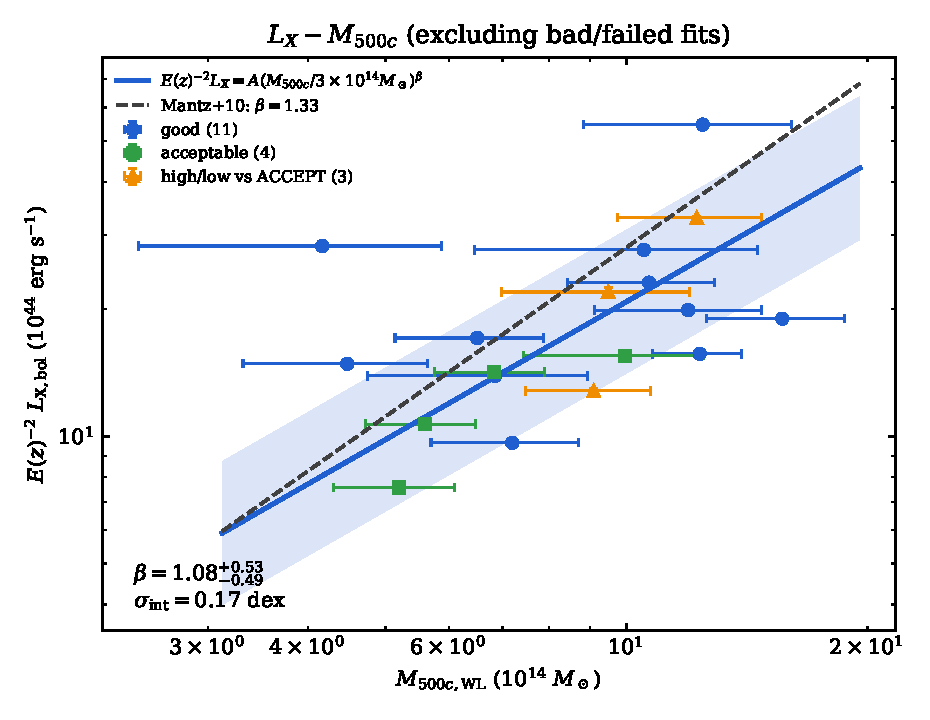
\includegraphics[width=\linewidth]{output/figures/scaling/lx_m500_linmix_exclude_bad.pdf}
    \caption{\Lx--\Mfive}
  \end{subfigure}
  \begin{subfigure}{0.48\linewidth}
    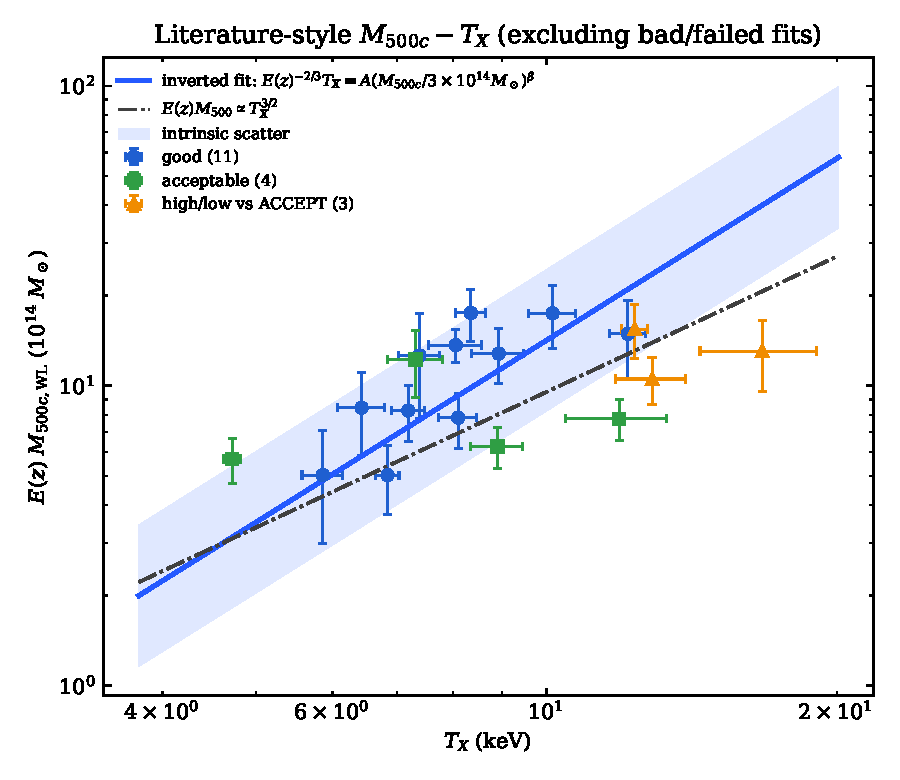
\includegraphics[width=\linewidth]{output/figures/scaling/m500_tx_literature_style_exclude_bad.pdf}
    \caption{\Tx--\Mfive}
  \end{subfigure}
  \begin{subfigure}{0.58\linewidth}
    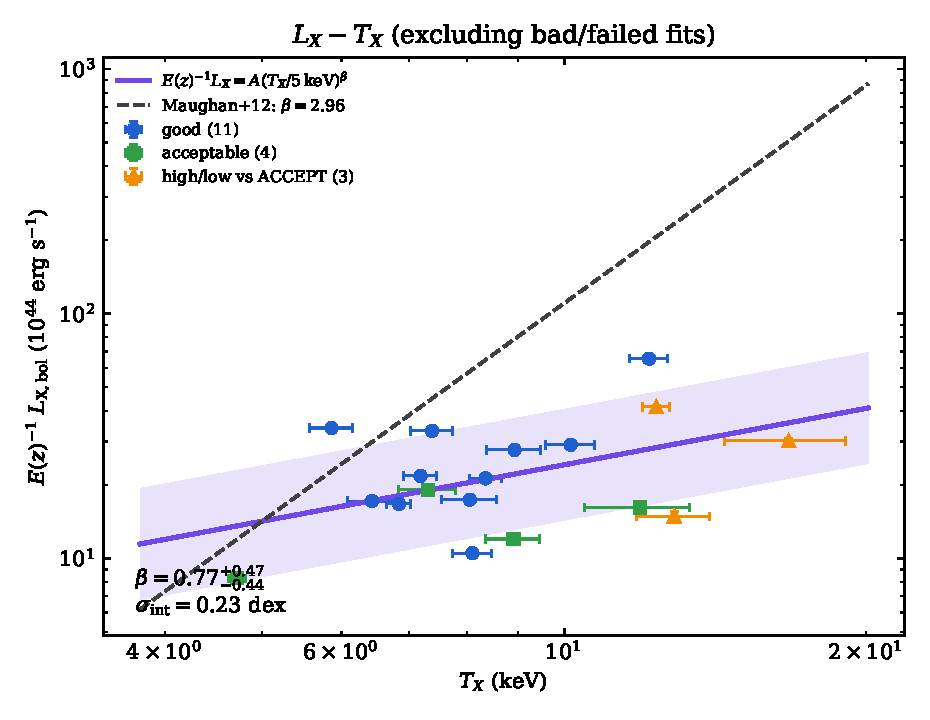
\includegraphics[width=\linewidth]{output/figures/scaling/lx_tx_linmix_exclude_bad.pdf}
    \caption{\Lx--\Tx}
  \end{subfigure}
  \caption{Full-\Rfive{} baseline scaling relations for the 18-cluster \texttt{exclude\_bad} sample.}
  \label{fig:full-scaling}
\end{figure}

\subsection{Core-Excised Comparison}

The core-excised branch measures the same retained 18 clusters over $0.15$--$1.0\Rfive$. Figure~\ref{fig:core-scaling} shows the corresponding fits. The core-excised \Lx--\Mfive{} slope is $\beta=1.15^{+0.54}_{-0.51}$ with scatter 0.186 dex, and the \Tx--\Mfive{} slope is $\beta=0.55^{+0.36}_{-0.34}$ with scatter 0.157 dex. The \Lx--\Tx{} slope is $\beta=0.69^{+0.40}_{-0.41}$ with scatter 0.245 dex. These values agree with the full-\Rfive{} mass-based slopes within the statistical uncertainties. In this small heterogeneous sample, core excision does not reduce the measured scatter; the likely reasons are sample size, retained high-temperature systems, heterogeneous Chandra coverage, and the temporary 10 percent \Tx{} uncertainty fallback in the core-excised branch.

\begin{figure}[p]
  \centering
  \begin{subfigure}{0.48\linewidth}
    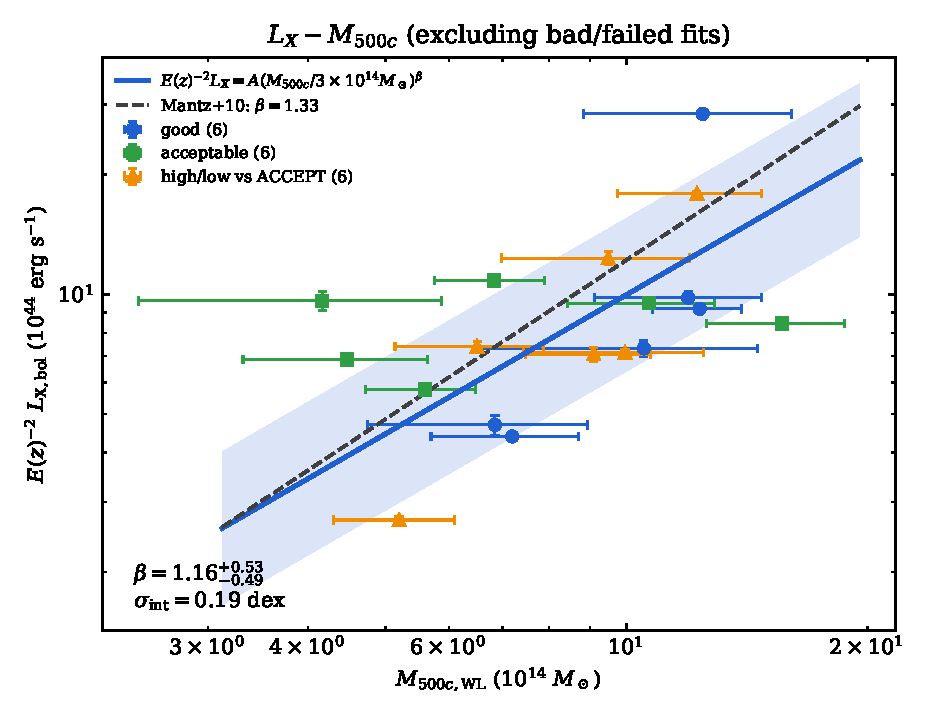
\includegraphics[width=\linewidth]{output/figures/scaling/core_excised/lx_m500_linmix_exclude_bad.pdf}
    \caption{\Lx--\Mfive}
  \end{subfigure}
  \begin{subfigure}{0.48\linewidth}
    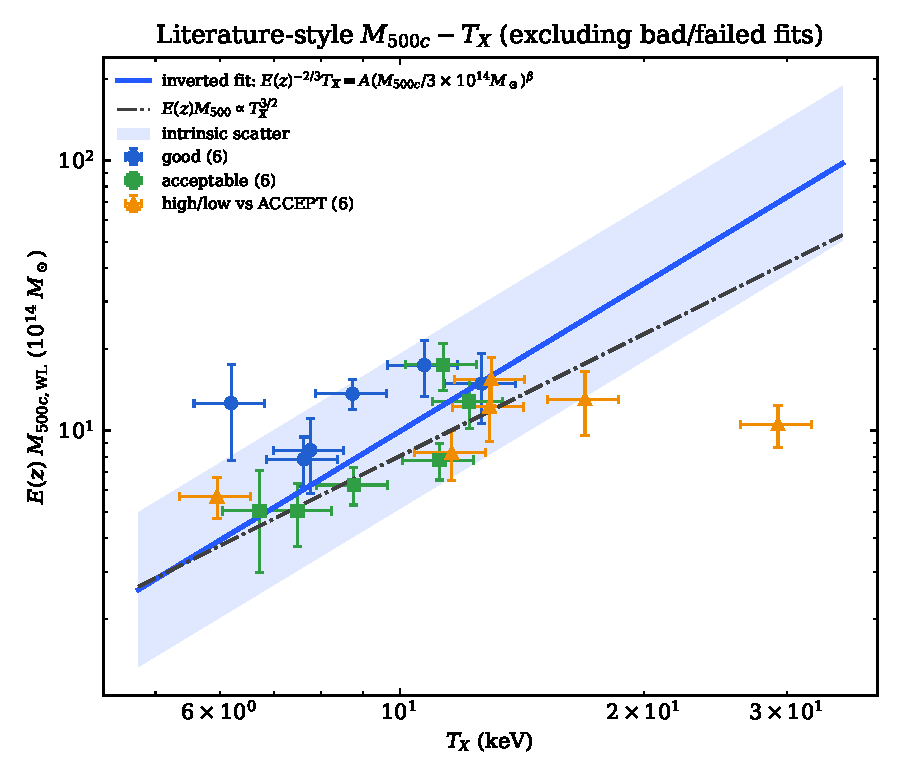
\includegraphics[width=\linewidth]{output/figures/scaling/core_excised/m500_tx_literature_style_exclude_bad.pdf}
    \caption{\Tx--\Mfive}
  \end{subfigure}
  \begin{subfigure}{0.58\linewidth}
    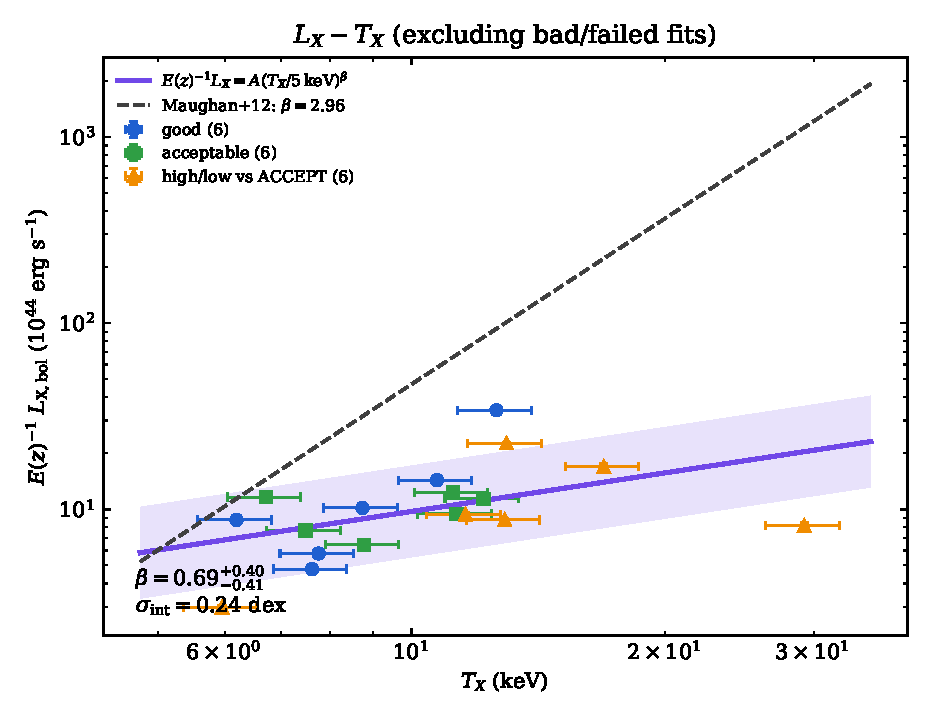
\includegraphics[width=\linewidth]{output/figures/scaling/core_excised/lx_tx_linmix_exclude_bad.pdf}
    \caption{\Lx--\Tx}
  \end{subfigure}
  \caption{Core-excised $0.15$--$1.0\Rfive$ scaling relations for the same 18-cluster \texttt{exclude\_bad} sample.}
  \label{fig:core-scaling}
\end{figure}

\begin{table}[t]
\centering
\caption{Main scaling results for the \texttt{exclude\_bad} sample.}
\label{tab:scaling}
\begin{tabular}{llcccc}
\toprule
Aperture & Relation & $N$ & $\beta$ & Intrinsic scatter & Note \\
 & & & & (dex) & \\
\midrule
Full \Rfive{} & \Lx--\Mfive{} & 18 & $1.08^{+0.45}_{-0.48}$ & 0.169 & Baseline \\
Full \Rfive{} & \Tx--\Mfive{} & 18 & $0.50^{+0.29}_{-0.27}$ & 0.117 & Baseline \\
Full \Rfive{} & \Lx--\Tx{} & 18 & $0.77^{+0.47}_{-0.44}$ & 0.227 & Noisiest relation \\
$0.15$--$1.0\Rfive$ & \Lx--\Mfive{} & 18 & $1.15^{+0.54}_{-0.51}$ & 0.186 & Core-excised \\
$0.15$--$1.0\Rfive$ & \Tx--\Mfive{} & 18 & $0.55^{+0.36}_{-0.34}$ & 0.157 & 10\% core \Tx{} fallback \\
$0.15$--$1.0\Rfive$ & \Lx--\Tx{} & 18 & $0.69^{+0.40}_{-0.41}$ & 0.245 & 10\% core \Tx{} fallback \\
\bottomrule
\end{tabular}
\end{table}

\subsection{Quality and Sensitivity}

The excluded systems are quality-control failures, not non-detections. Abell 0697 and MS2137--2353 produce extreme temperatures and poor fit behavior; Abell 0750 has a poor early-data fit; RXJ1347.5--1145 worsens when all available ObsIDs are included; and ZwCl 0857.9+2107 appears inconsistent with the external ACCEPT reference/aperture comparison. Leaving these clusters in the headline regression would make the result a statement about failed spectra rather than cluster scaling.

The retained high/suspect systems were tested with leave-one-out refits. Removing Abell 0068, Abell 0611, MACSJ0647.7+7015, or MACSJ1206.2--0847 shifts the \Lx--\Mfive{} and \Tx--\Mfive{} slopes by less than the current statistical error. The \Lx--\Tx{} relation is more sensitive, especially to Abell 0611 and MACSJ1206.2--0847, reinforcing the decision to treat it as a consistency relation rather than the headline result.

\section{Discussion}

The full-\Rfive{} and core-excised mass-based slopes agree within the current uncertainties. This stability is encouraging: it suggests that the main mass calibration is not driven purely by cool-core emission, despite the heterogeneous sample. At the same time, the scatter does not improve after core excision, unlike in some larger and more controlled literature samples \citep{pratt2009,mantz2010,mantz2016}. This difference should not be over-interpreted. The present project has only 18 clusters in the baseline fit, a mix of CLASH and LoCuSS selection, non-uniform Chandra depth, several high-temperature retained systems, and a known core-excised \Tx{} error fallback.

Compared with the literature, the \Tx--\Mfive{} slope is broadly compatible with self-similar expectations and with the idea that temperature is a relatively low-scatter mass proxy. The \Lx--\Mfive{} slope is lower than many steep luminosity--mass measurements but is consistent with self-similar within the large uncertainty. The shallow \Lx--\Tx{} slope is the least robust result and likely reflects the combination of temperature outliers, small dynamic range, and measurement covariance. A publication-level version should strengthen the background QA, fill missing confidence intervals, and eventually use a hierarchical model with explicit selection effects if the sample definition is expanded.

\section{Conclusions}

\begin{enumerate}
\item The project reproduces a full Chandra-to-scaling-relation workflow: CIAO reprocessing, point-source masking, per-ObsID spectra, Sherpa WSTAT fits, canonical spectral tables, and \texttt{linmix} regressions.
\item The final main sample contains 18 weak-lensing calibrated CLASH+LoCuSS clusters after excluding five bad or failed spectral objects.
\item The full-\Rfive{} baseline gives $\beta_{\Lx-M}=1.08^{+0.45}_{-0.48}$ and $\beta_{\Tx-M}=0.50^{+0.29}_{-0.27}$, with intrinsic scatter 0.169 dex and 0.117 dex.
\item The core-excised branch gives consistent mass-based slopes, so the current scientific conclusion is stable to core excision at the available precision.
\item The \Lx--\Tx{} relation remains shallow and noisy and should be treated as a sensitivity-limited consistency check rather than the primary result.
\end{enumerate}

\appendix
\section{20-Minute Presentation Guide}

This report can be used as a speaking reference with the following timing. The goal is not to read every paragraph, but to keep the causal story visible while presenting the figures.

\begin{table}[ht]
\centering
\caption{Suggested oral-report structure.}
\begin{tabular}{p{0.13\linewidth}p{0.25\linewidth}p{0.52\linewidth}}
\toprule
Time & Section & Main speaking point \\
\midrule
2 min & Motivation & Clusters connect cosmology and baryonic physics; X-ray gas is a mass tracer because it lives in the cluster potential. \\
4 min & Physical scaling logic & Walk through Figure~\ref{fig:physical-chain}: \Mfive{} sets potential depth, potential sets \Tx{} and gas density, gas produces \Lx{}, and real clusters add intrinsic scatter. \\
4 min & Sample/workflow & Explain the CLASH+LoCuSS parent sample, the 23 processed clusters, the 18-cluster main sample, and why per-ObsID spectral responses matter. \\
5 min & Spectral model & Emphasize absorbed APEC, WSTAT, blank-sky 9.5--12 keV renormalization, XRB components, and why background control is the dominant technical risk. \\
3 min & Scaling results & Focus on the full-\Rfive{} \Lx--\Mfive{} and \Tx--\Mfive{} slopes, then use the core-excised branch as a stability check. \\
2 min & Limitations and conclusion & State that mass-based slopes are stable within uncertainty, while \Lx--\Tx{} is noisy; future improvements need better confidence intervals and background QA. \\
\bottomrule
\end{tabular}
\end{table}

The simplest closing sentence is: this project shows that Chandra-measured hot-gas observables trace weak-lensing halo mass in the expected broad sense, but the precision is currently limited by small-sample statistics, heterogeneous data quality, and background-sensitive spectral modeling.

\section{Retained Cluster Spectral Table}

\begin{longtable}{lrrrrrr}
\caption{Retained 18-cluster sample. Luminosities are bolometric in $10^{44}\,\mathrm{erg\,s^{-1}}$.}\\
\toprule
Cluster & $z$ & $M_{500}$ & $T_{\rm full}$ & $L_{\rm full}$ & $T_{\rm core}$ & $L_{\rm core}$ \\
 & & ($10^{14}M_\odot$) & (keV) & & (keV) & \\
\midrule
\endfirsthead
\toprule
Cluster & $z$ & $M_{500}$ & $T_{\rm full}$ & $L_{\rm full}$ & $T_{\rm core}$ & $L_{\rm core}$ \\
 & & ($10^{14}M_\odot$) & (keV) & & (keV) & \\
\midrule
\endhead
Abell 0209 & 0.206 & 12.34 & 8.05 & 19.22 & 8.74 & 11.26 \\
Abell 0068 & 0.255 & 6.83 & 11.90 & 18.34 & 11.19 & 13.99 \\
Abell 0267 & 0.230 & 5.60 & 8.90 & 13.45 & 8.77 & 7.24 \\
Abell 0383 & 0.187 & 5.20 & 4.72 & 9.09 & 5.95 & 3.25 \\
Abell 0586 & 0.171 & 7.20 & 8.10 & 11.41 & 7.62 & 5.19 \\
Abell 0611 & 0.288 & 9.10 & 12.87 & 17.18 & 29.23 & 9.47 \\
Abell 2261 & 0.224 & 15.65 & 8.35 & 23.73 & 11.30 & 10.56 \\
MACSJ0329.7--0211 & 0.450 & 6.51 & 7.19 & 27.58 & 11.58 & 11.94 \\
MACSJ0429.6--0253 & 0.399 & 6.85 & 6.43 & 21.14 & 7.75 & 7.14 \\
MACSJ0647.7+7015 & 0.584 & 9.49 & 16.74 & 41.54 & 16.90 & 23.33 \\
MACSJ0744.9+3927 & 0.686 & 11.94 & 10.15 & 42.52 & 10.72 & 20.95 \\
MACSJ1115.9+0129 & 0.352 & 10.67 & 8.92 & 33.31 & 12.17 & 13.68 \\
MACSJ1206.2--0847 & 0.440 & 12.24 & 12.35 & 52.51 & 12.96 & 28.60 \\
MACSJ1720.3+3536 & 0.391 & 9.96 & 7.32 & 23.38 & 12.89 & 10.76 \\
MACSJ1931.8--2635 & 0.352 & 10.51 & 7.39 & 39.81 & 6.20 & 10.54 \\
RXJ1532.9+3021 & 0.363 & 4.17 & 5.86 & 41.16 & 6.71 & 14.04 \\
RXJ2129.7+0005 & 0.234 & 4.48 & 6.84 & 18.76 & 7.48 & 8.67 \\
RXJ2248.7--4431 & 0.348 & 12.45 & 12.15 & 78.38 & 12.61 & 40.77 \\
\bottomrule
\end{longtable}

\bibliographystyle{plainnat}
\bibliography{references}

\end{document}
